\documentclass[border=3pt]{standalone}
% Preâmbulo compartilhado pelos diagramas TikZ da aula 4 de Navegação (Representação de Mapas)
\usepackage[T1]{fontenc}
\usepackage[utf8]{inputenc}
\usepackage{lmodern}
\usepackage{amsmath}
\usepackage{xcolor}
\usepackage{tikz}
\usetikzlibrary{arrows.meta,angles,quotes,decorations.pathmorphing,decorations.pathreplacing,calc,
                positioning,shapes.geometric,shapes.misc,backgrounds,fit,
                math}

% Paleta (mesma dos SVGs originais)
\definecolor{dblue}{HTML}{2A5B8C}
\definecolor{dorange}{HTML}{B3541E}
\definecolor{dgreen}{HTML}{4A7C59}
\definecolor{dred}{HTML}{9C4B4B}
\definecolor{dcream}{HTML}{F4F1EA}
\definecolor{dshade}{HTML}{DDD7C9}

% Função gaussiana (não normalizada por padrão de escala visual)
\pgfmathdeclarefunction{gauss}{3}{%
  \pgfmathparse{1/(#3*sqrt(2*pi))*exp(-((#1-#2)^2)/(2*#3^2))}%
}

% Estilos comuns (prefixo d... para não colidir com chaves internas do pgf)
\tikzset{
  >={Stealth[length=2mm]},
  dguide/.style={gray!55, dashed, line width=0.4pt},
  daxis/.style={gray!60, line width=0.7pt, ->},
  dbody/.style={fill=black!3, draw=black!80, line width=1pt},
  dacc/.style={draw=dblue, line width=1pt},
  dlbl/.style={black!55, font=\small},
  dsub/.style={black!45, font=\footnotesize},
  dstate/.style={circle, draw=black!80, fill=dcream, line width=1pt,
                 minimum size=17mm, font=\large, inner sep=1pt},
  dobs/.style={circle, draw=black!80, fill=dshade, line width=1pt,
               minimum size=14mm, font=\large, inner sep=1pt},
  dbox/.style={rounded corners=2pt, draw=black!80, fill=dcream, line width=1pt,
               align=center, inner sep=6pt},
  dop/.style={circle, draw=black!80, fill=white, line width=1pt,
              minimum size=6mm, inner sep=0pt, font=\small},
  dtrans/.style={->, dblue, line width=1pt},
  dmeas/.style={->, dorange, line width=1pt},
  dcurve/.style={line width=1pt, dblue},
  dcurveb/.style={line width=1.4pt, dorange},
}

\begin{document}
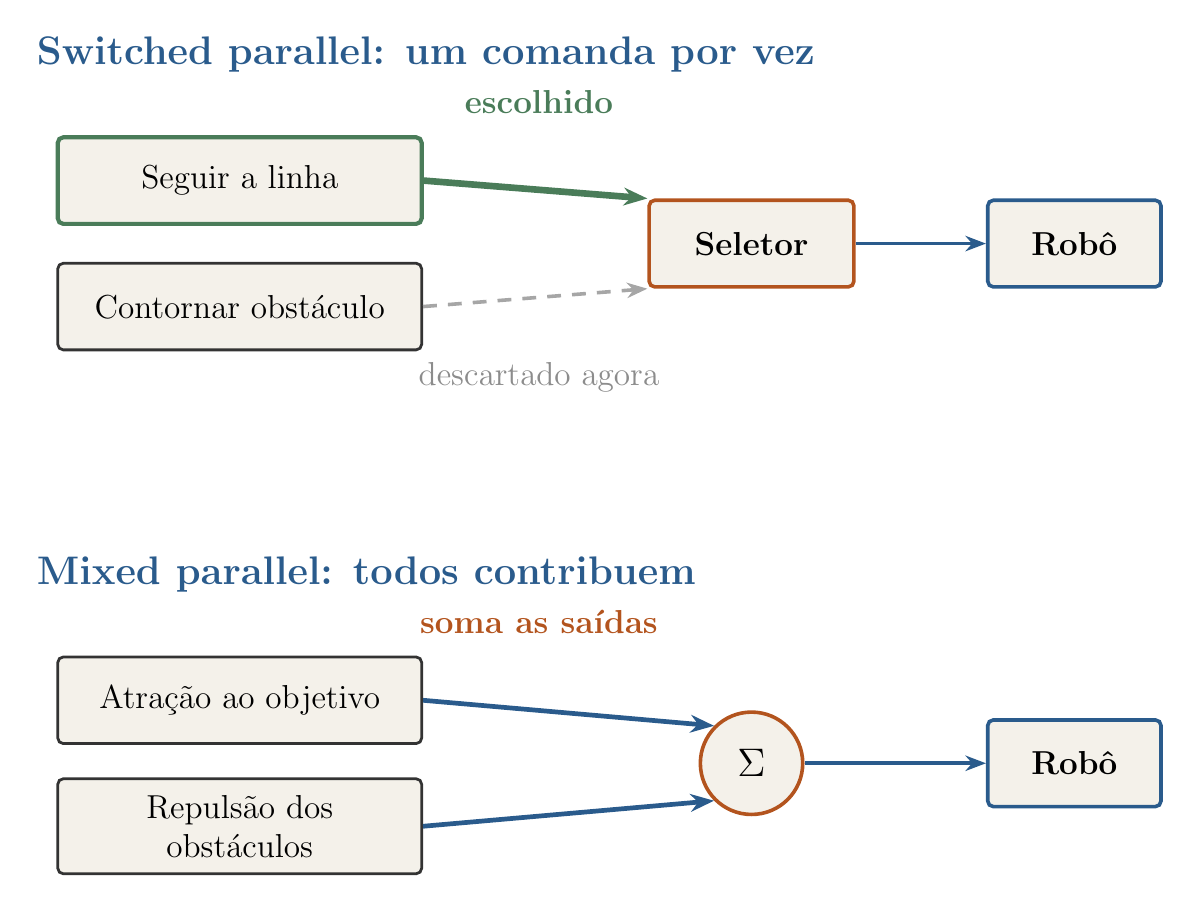
\begin{tikzpicture}[x=1cm,y=1cm]

  \tikzset{mod/.style={dbox, minimum width=4.2cm, text width=4.2cm, minimum height=1.1cm, font=\large, align=center},
           rob/.style={dbox, minimum width=2.2cm, minimum height=1.1cm, font=\large\bfseries, draw=dblue, line width=1.3pt},
           sel/.style={dbox, minimum width=2.6cm, minimum height=1.1cm, font=\large\bfseries, draw=dorange, line width=1.3pt},
           soma/.style={circle, draw=dorange, fill=dcream, line width=1.3pt, minimum size=1.3cm, font=\Large\bfseries}}

  % ---------- Switched parallel ----------
  \node[font=\bfseries\Large, dblue, anchor=west] at (-0.6,5.5) {Switched parallel: um comanda por vez};
  \node[mod, draw=dgreen, line width=1.5pt] (s1) at (2.1,3.9) {Seguir a linha};
  \node[mod] (s2) at (2.1,2.3) {Contornar obstáculo};
  \node[sel] (sw) at (8.6,3.1) {Seletor};
  \node[rob] (r1) at (12.7,3.1) {Robô};
  \draw[dgreen, line width=2.4pt, -{Stealth[length=3mm]}] (s1.east) -- (sw.north west);
  \draw[black!35, line width=1.3pt, dash pattern=on 5pt off 4pt, -{Stealth[length=2.6mm]}] (s2.east) -- (sw.south west);
  \draw[dtrans, line width=1.3pt, -{Stealth[length=2.6mm]}] (sw) -- (r1);
  \node[dgreen, font=\large\bfseries, align=center] at (5.9,4.9) {escolhido};
  \node[black!45, font=\large, align=center] at (5.9,1.4) {descartado agora};

  % ---------- Mixed parallel ----------
  \begin{scope}[shift={(0,-6.6)}]
  \node[font=\bfseries\Large, dblue, anchor=west] at (-0.6,5.5) {Mixed parallel: todos contribuem};
  \node[mod] (m1) at (2.1,3.9) {Atração ao objetivo};
  \node[mod] (m2) at (2.1,2.3) {Repulsão dos obstáculos};
  \node[soma] (sm) at (8.6,3.1) {$\Sigma$};
  \node[rob] (r2) at (12.7,3.1) {Robô};
  \draw[dtrans, line width=1.7pt, -{Stealth[length=3mm]}] (m1.east) -- (sm.north west);
  \draw[dtrans, line width=1.7pt, -{Stealth[length=3mm]}] (m2.east) -- (sm.south west);
  \draw[dtrans, line width=1.3pt, -{Stealth[length=2.6mm]}] (sm) -- (r2);
  \node[dorange, font=\large\bfseries, align=center] at (5.9,4.9) {soma as saídas};
  \end{scope}

\end{tikzpicture}
\end{document}
